%%%% Compilare con pdflatex %%%%%%%%%%%%%%%%
\documentclass[a4paper,10pt]{report}
% Package(s) to include
\usepackage{textcomp}
\usepackage{graphicx}
\title{wxGlade 2.0 user manual}
\author{Marcello Semboli}

%%%%%%%%%%%%%%%%%% END OF PREAMBULE %%%%%%%%%%%%%%%%%%

\pagestyle{empty}
\begin{document}

\maketitle
\tableofcontents

\chapter{Preface}
This manual describes the wxGlade version 0.2.2, a Python, Perl,  C++
and XRC Graphical User Interface ("GUI") Editor for UNIX and
Microsoft Windows. Each of the chapters in this manual is designed
as a tutorial for using wxGlade and a referense for widgets
supported until now.


\section{Abbreviations}
The following abbreviations are used in this manual:

\begin{itemize}
\item
\emph{X11} - The X Window System version 11.
\item
\emph{wx} - The wxWindows open source C++ GUI framework.
\item
\emph{WIN32} - The Microsoft Windows 32-bit Application Programmer's Interface.
\end{itemize}

\section{Contacts}
Informations, support and bug reports can be addressed to the
wxGlade mailing list:
wxglade-general@lists.sourceforge.net.

The mantainer of this document is Marcello Semboli.
You can address any message regarding this document to "Marcello
Semboli" \textless\{\}dinogen@siena.linux.it\textgreater\{\}.

\section{Copyrights and Trademarks}
wxGlade is Copyright 2002-2003 by Alberto Griggio. Use and distribution
of wxGlade is governed by the MIT license, located in Appendix A.

wxWindows is Copyright (c) 1992-2002 Julian Smart, Robert Roebling,
Vadim Zeitlin and other members of the wxWindows team.
See: http://www.wxwindows.org for details.

UNIX is a registered trademark of the X Open Group, Inc.

Microsoft and Windows are registered trademarks of Microsoft
Corporation.
%\newpage


\chapter{Introduction to wxGlade}

\section{What wxGlade is }

wxGlade is a GUI designer written in Python with the popular
GUI toolkit wxPython, that helps you create wxWindows/wxPython
user interfaces. At the moment it can generate Python, C++ and
XRC (wxWindows' XML resources) code.

As you can guess by the name, its model is Glade, the famous
GTK+/GNOME GUI builder, with which wxGlade shares the philosophy
and the look \&\{\} feel (but not a line of code).


\section{What wxGlade is NOT}

It is not (and will never be) a full featured IDE, but simply
a "designer": the generated code does nothing apart from displaying
the created widgets. If you are looking for a complete IDE,
maybe Boa Constructor (http://boa-constructor.sourceforge.net/)
or PythonCard (http://www.pythoncard.org/) is the right tool.



\section{Download}
You can download source files for the stable version from the
sourceforge project page (http://sourceforge.net/projects/wxglade).


You can get the unstable version from Sourceforge anonymous CVS
access. Refer to Sourceforge CVS documentation for details.


Also binaries for Microsoft Windows and Linux are provided for
download.

\section{Installation and requirements}


While Python is a pseudo-interpreted language, you don't need
any "compile" or "make" steps.


wxGlade requires Python version 2.2 or later and wxPython version
2.3.2.1 or later.
The binary versions are stand-alone and doesn't have any requirement.
\section{Basics}

You need to know basics of wxWindows or wxPython.
Also you need basics of C++ or Python or Perl.
You can't use wxGlade if you have not any basic of programming.
You can't learn wx programming reading this manual, as well.

\section{Contacts}
Check in the sourceforge project page (http://sourceforge.net/projects/wxglade)
for the mailing list to discuss about the project.
Use the lists for questions, proposal, bug reports and collaboration.

If you don't want to follow the list, you can reach me at albgrig@tiscalinet.it:
any kind of feedback is always welcome.

\chapter{Exploring wxGlade}

\section{Quick start}

We will design a simple form.

Start wxGlade running wxglade.py program.

You will see a Main Window, with several buttons, and a Tree
Window with a icon "Application".  A Properties Window is showing
properties of the Application.


If you move the mouse over a main window's button, a tooltip
display the function of the button.


To add a frame at the design window, from the Main Window choose
the first button: "Add a frame".

Then choose wxFrame as base class.

Look at the tree window and see that two icons are generated
under the application icon, a frame icon and a sizer icon.

If you double click with the mouse on the frame icon, the designer
window appears.
Notice that the sizer is displayed as a set of gray boxes: they are
the "slots" of the grid sizer where you will place the widgets.

You put a widgets on a sizer by selecting it on the Main Window,
then click on a empty slot on the frame on the designer window.
Try adding a static text, a text control and a button.
If you want add something else, add empty slots on the sizer by
right-click on the sizer on the tree window and selecting "Add slot".
Play adding four or five widgets on the frame.

Now look at the properties form; there are three tabs. In the "Common"
tab you can specify name, size and color of the widget.
In the "Layout" tab you can adjust borders and alignements.
In the "Widget" tab you find the properties depending to the
widget.

You can select the properties of a widget by clicking on the designer window
or the corresponding icon on the tree window.
Try adjusting widgets with the properties form until you know you
played enougth.

Now let's generate the code.

Select the Application icon on the tree window and
pay attention to the properties window;
Check Name and Class, choose a Top window, check Single file and
choose the language
and set the Output path pushing the button for selecting a path and a filename.
Finally press the Generate code button and the code is generate.

Compile and enjoy.


\section{Basics of wxGlade}

The program wxGlade is a tool for designing Graphical User Interface (GUI).
It is intended to use with wxWindows framework in all its flawors: C++, Perl, 
Python and XRC.
You use a visual editor for creating forms, menus and toolbars with the mouse.
Your design is saved in a .wxg file that is the wxGlade file format.
Then you generate source code or XRC by using visual tools or invoking wxGlade 
in the command line.
You can also use wxGlade in your makefile generating source code only when the .wxg
change.
A .wxg file can contains multiple forms, panels, menus and toolbars and generate 
a single file containing all classes or multiple files containing one class each.

\section{Using the source code}

How do you use source code generated by wxGlade? Basically in two ways.

You can safely edit the source code of the generated class. This because
wxGlade mark the untouchable code with the special comments "begin wxGlade" and "end wxGlade".
So you can edit all you need outside these two tags. When you makes 
changes in your forms, a new code generation will not modify the user code.

The other way is to generate the class with wxGlade in a file (e.g. myFormUI.xxx) and 
subclass it in another file (e.g. myForm.xxx). This give you the psychological advantage
that there is a file for you a one for wxGlade :-) .

\chapter{wxGlade User Interface}

\section{Main Window}

The main window hosts the menu and the widgets choice buttons.

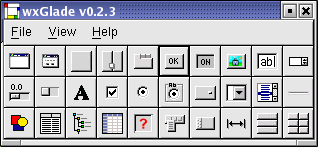
\includegraphics{manual_main.png}

If you pass the mouse pointer on a button a tooltip show the button's 
description.

The ``frame'' button and the ``Dialog'' button show up a dialog
to add a frame, a dialog or a panel to your project.

Other buttons in the main window adds widgets in a form. 
When you click on such button, 
the cursor pointer change in an arrow, then you can click on
a sizer's empty cell and add the widget to it.
 

 
%%%%%%% APPENDIX %%%%%%%%%%%%%%%%%%%%%%%%%%%%%%%%

\appendix

\chapter{Appendix A: MIT License}
Copyright (c) 2002-2003 Alberto Griggio  albgrig@tiscalinet.it.

Permission is hereby granted, free of charge, to any person obtaining
a copy of
this software and associated documentation files (the "Software"),
to deal in
the Software without restriction, including without limitation
the rights to
use, copy, modify, merge, publish, distribute, sublicense, and/or
sell copies
of the Software, and to permit persons to whom the Software is
furnished to do
so, subject to the following conditions:

The above copyright notice and this permission notice shall be
included in all
copies or substantial portions of the Software.

THE SOFTWARE IS PROVIDED "AS IS", WITHOUT WARRANTY OF ANY KIND,
EXPRESS OR IMPLIED, INCLUDING BUT NOT LIMITED TO THE WARRANTIES
OF MERCHANTABILITY, FITNESS FOR A PARTICULAR PURPOSE AND NONINFRINGEMENT.
IN NO EVENT SHALL THE AUTHORS OR COPYRIGHT HOLDERS BE LIABLE
FOR ANY CLAIM, DAMAGES OR OTHER LIABILITY, WHETHER IN AN ACTION
OF CONTRACT, TORT OR OTHERWISE, ARISING FROM, OUT OF OR IN CONNECTION
WITH THE SOFTWARE OR THE USE OR OTHER DEALINGS IN THE SOFTWARE.


\end{document}

